\section{Hasil \& Evaluasi}

\begin{frame}{Hasil Evaluasi Akhir Keseluruhan}
    \begin{center}
        \small
        \begin{tabular}{lcc}
            \toprule
            \textbf{Skenario Model / Baseline} & \textbf{WER (\%)} & \textbf{CER (\%)} \\
            \midrule
            Zero-Shot Whisper Original & 89,44 & 31,02 \\
            \textbf{Freeze Encoder Terbaik (run\_20260303\_202534)} & \textbf{18,24 $\pm$ 2,18} & \textbf{3,87 $\pm$ 0,61} \\
            \midrule
            \textbf{LoRA Terbaik (lora\_20260305\_205845)} & \textbf{15,67 $\pm$ 1,02} & \textbf{3,32 $\pm$ 0,38} \\
            \bottomrule
        \end{tabular}
    \end{center}
    \vspace{0.2cm}
    \begin{itemize}
        \item Kriteria pemilihan run terbaik: \textbf{mean WER paling kecil} pada 5-fold cross-validation (tie-breaker: mean CER).
        \item Perbaikan terhadap \textit{zero-shot}: Freeze Encoder turun \textbf{79,61\%} dan LoRA turun \textbf{82,48\%} pada WER.
        \item LoRA memberi nilai rata-rata error terbaik sekaligus simpangan antar-fold yang lebih kecil dibanding Freeze Encoder.
    \end{itemize}
\end{frame}

\begin{frame}{Rincian Performa Tiap Fold (Run Terbaik FE vs LoRA)}
    \begin{center}
        \scriptsize
        \begin{tabular}{lcccc}
            \toprule
            \textbf{Skenario Model} & \multicolumn{2}{c}{\textbf{Freeze Encoder (run\_20260303\_202534)}} & \multicolumn{2}{c}{\textbf{LoRA (lora\_20260305\_205845)}} \\
            \cmidrule(lr){2-3} \cmidrule(lr){4-5}
            \textbf{Partisi Lipatan} & \textbf{WER (\%)} & \textbf{CER (\%)} & \textbf{WER (\%)} & \textbf{CER (\%)} \\
            \midrule
            Fold Ke-1 (\#0) & 18,58 & 3,86 & 16,28 & 3,71 \\
            Fold Ke-2 (\#1) & \textbf{16,10} & 3,37 & 14,63 & 3,16 \\
            Fold Ke-3 (\#2) & 16,52 & \textbf{3,03} & \textbf{14,49} & \textbf{2,90} \\
            Fold Ke-4 (\#3) & 22,22 & 4,48 & 17,20 & 2,99 \\
            Fold Ke-5 (\#4) & 17,78 & 4,62 & 15,74 & 3,84 \\
            \midrule
            \textbf{Rata-rata/Mean $\pm$ Std} & \textbf{18,24 $\pm$ 2,18} & \textbf{3,87 $\pm$ 0,61} & \textbf{15,67 $\pm$ 1,02} & \textbf{3,32 $\pm$ 0,38} \\
            \bottomrule
        \end{tabular}
    \end{center}
    \vspace{0.2cm}
    \begin{itemize}
        \small
        \item Freeze Encoder terbaik di WER terjadi pada Fold \#1 (16,10\%), sedangkan CER terbaik terjadi pada Fold \#2 (3,03\%).
        \item LoRA memiliki WER dan CER terbaik pada Fold \#2 (14,49\% dan 2,90\%).
        \item Variasi hasil antar-fold pada LoRA lebih sempit sehingga performa lebih konsisten.
    \end{itemize}
\end{frame}

\begin{frame}{Komparasi Cross-Validation: FE Terbaik vs LoRA Terbaik}
    \begin{columns}
        \begin{column}{0.5\textwidth}
            \begin{figure}[!ht]
                \centering
                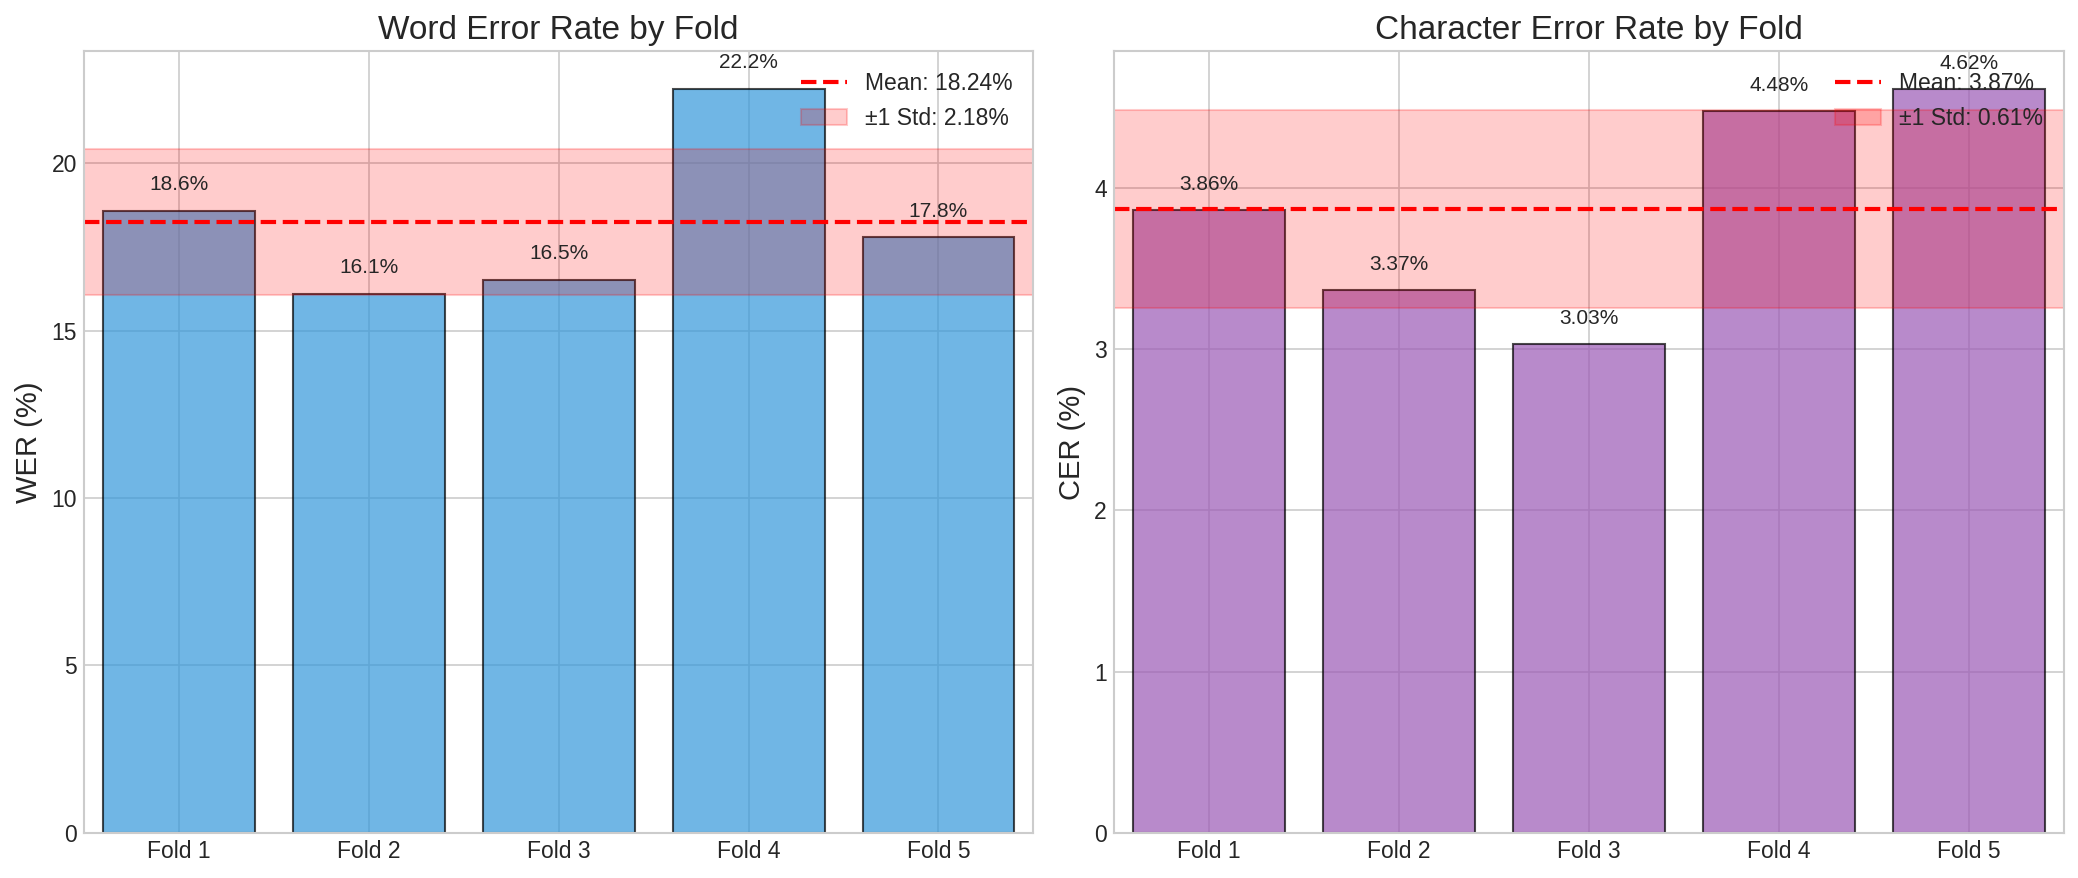
\includegraphics[width=\textwidth]{../code/freeze_encoder/outputs/metrics/run_20260303_202534/visualizations/cross_validation_summary.png}
                \caption{Distribusi WER, CER \& Waktu Evaluasi \textbf{FE terbaik}}
            \end{figure}
        \end{column}
        \begin{column}{0.5\textwidth}
            \begin{figure}[!ht]
                \centering
                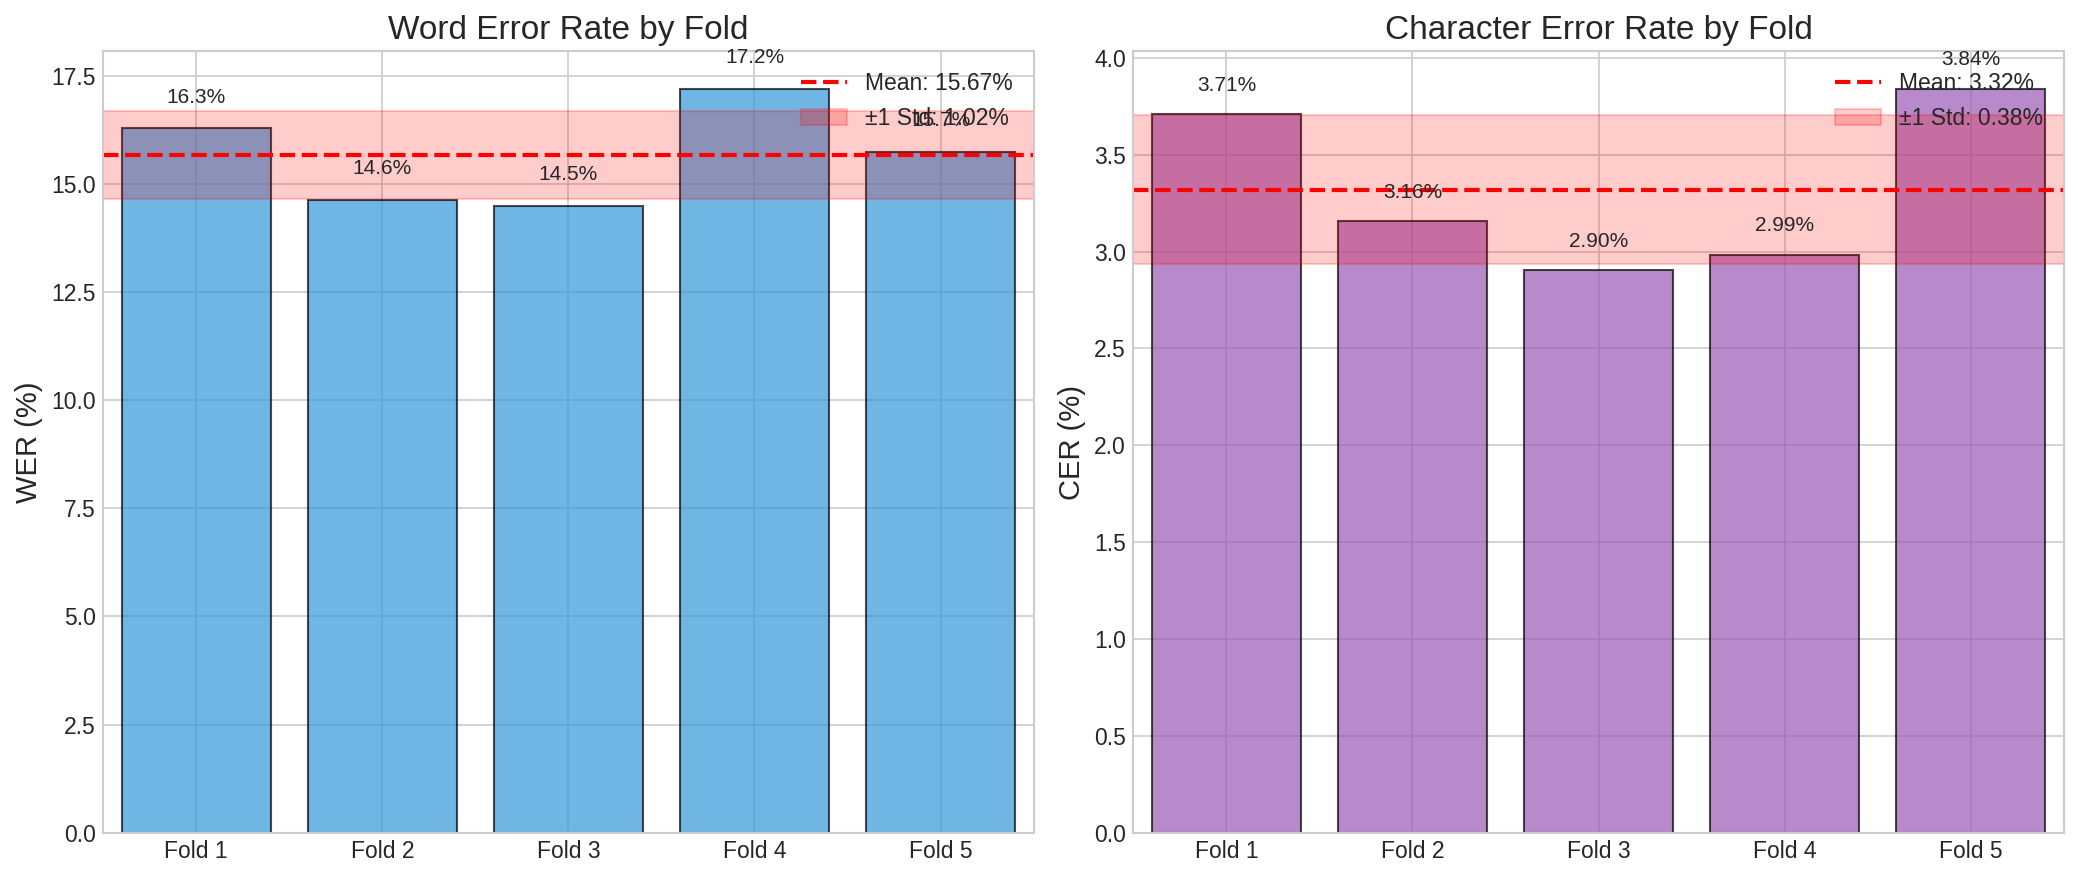
\includegraphics[width=\textwidth]{../code/lora/outputs/metrics/lora_20260305_205845/visualizations/cross_validation_summary.png}
                \caption{Distribusi WER, CER \& Waktu Evaluasi \textbf{LoRA terbaik}}
            \end{figure}
        \end{column}
    \end{columns}
\end{frame}

\begin{frame}{Dashboard Evaluasi Metrik Menyeluruh}
    \vspace{-0.2cm}
    \begin{columns}
        \begin{column}{0.5\textwidth}
            \textbf{Freeze Encoder (run\_20260303\_202534)}
            \begin{figure}
                \centering
                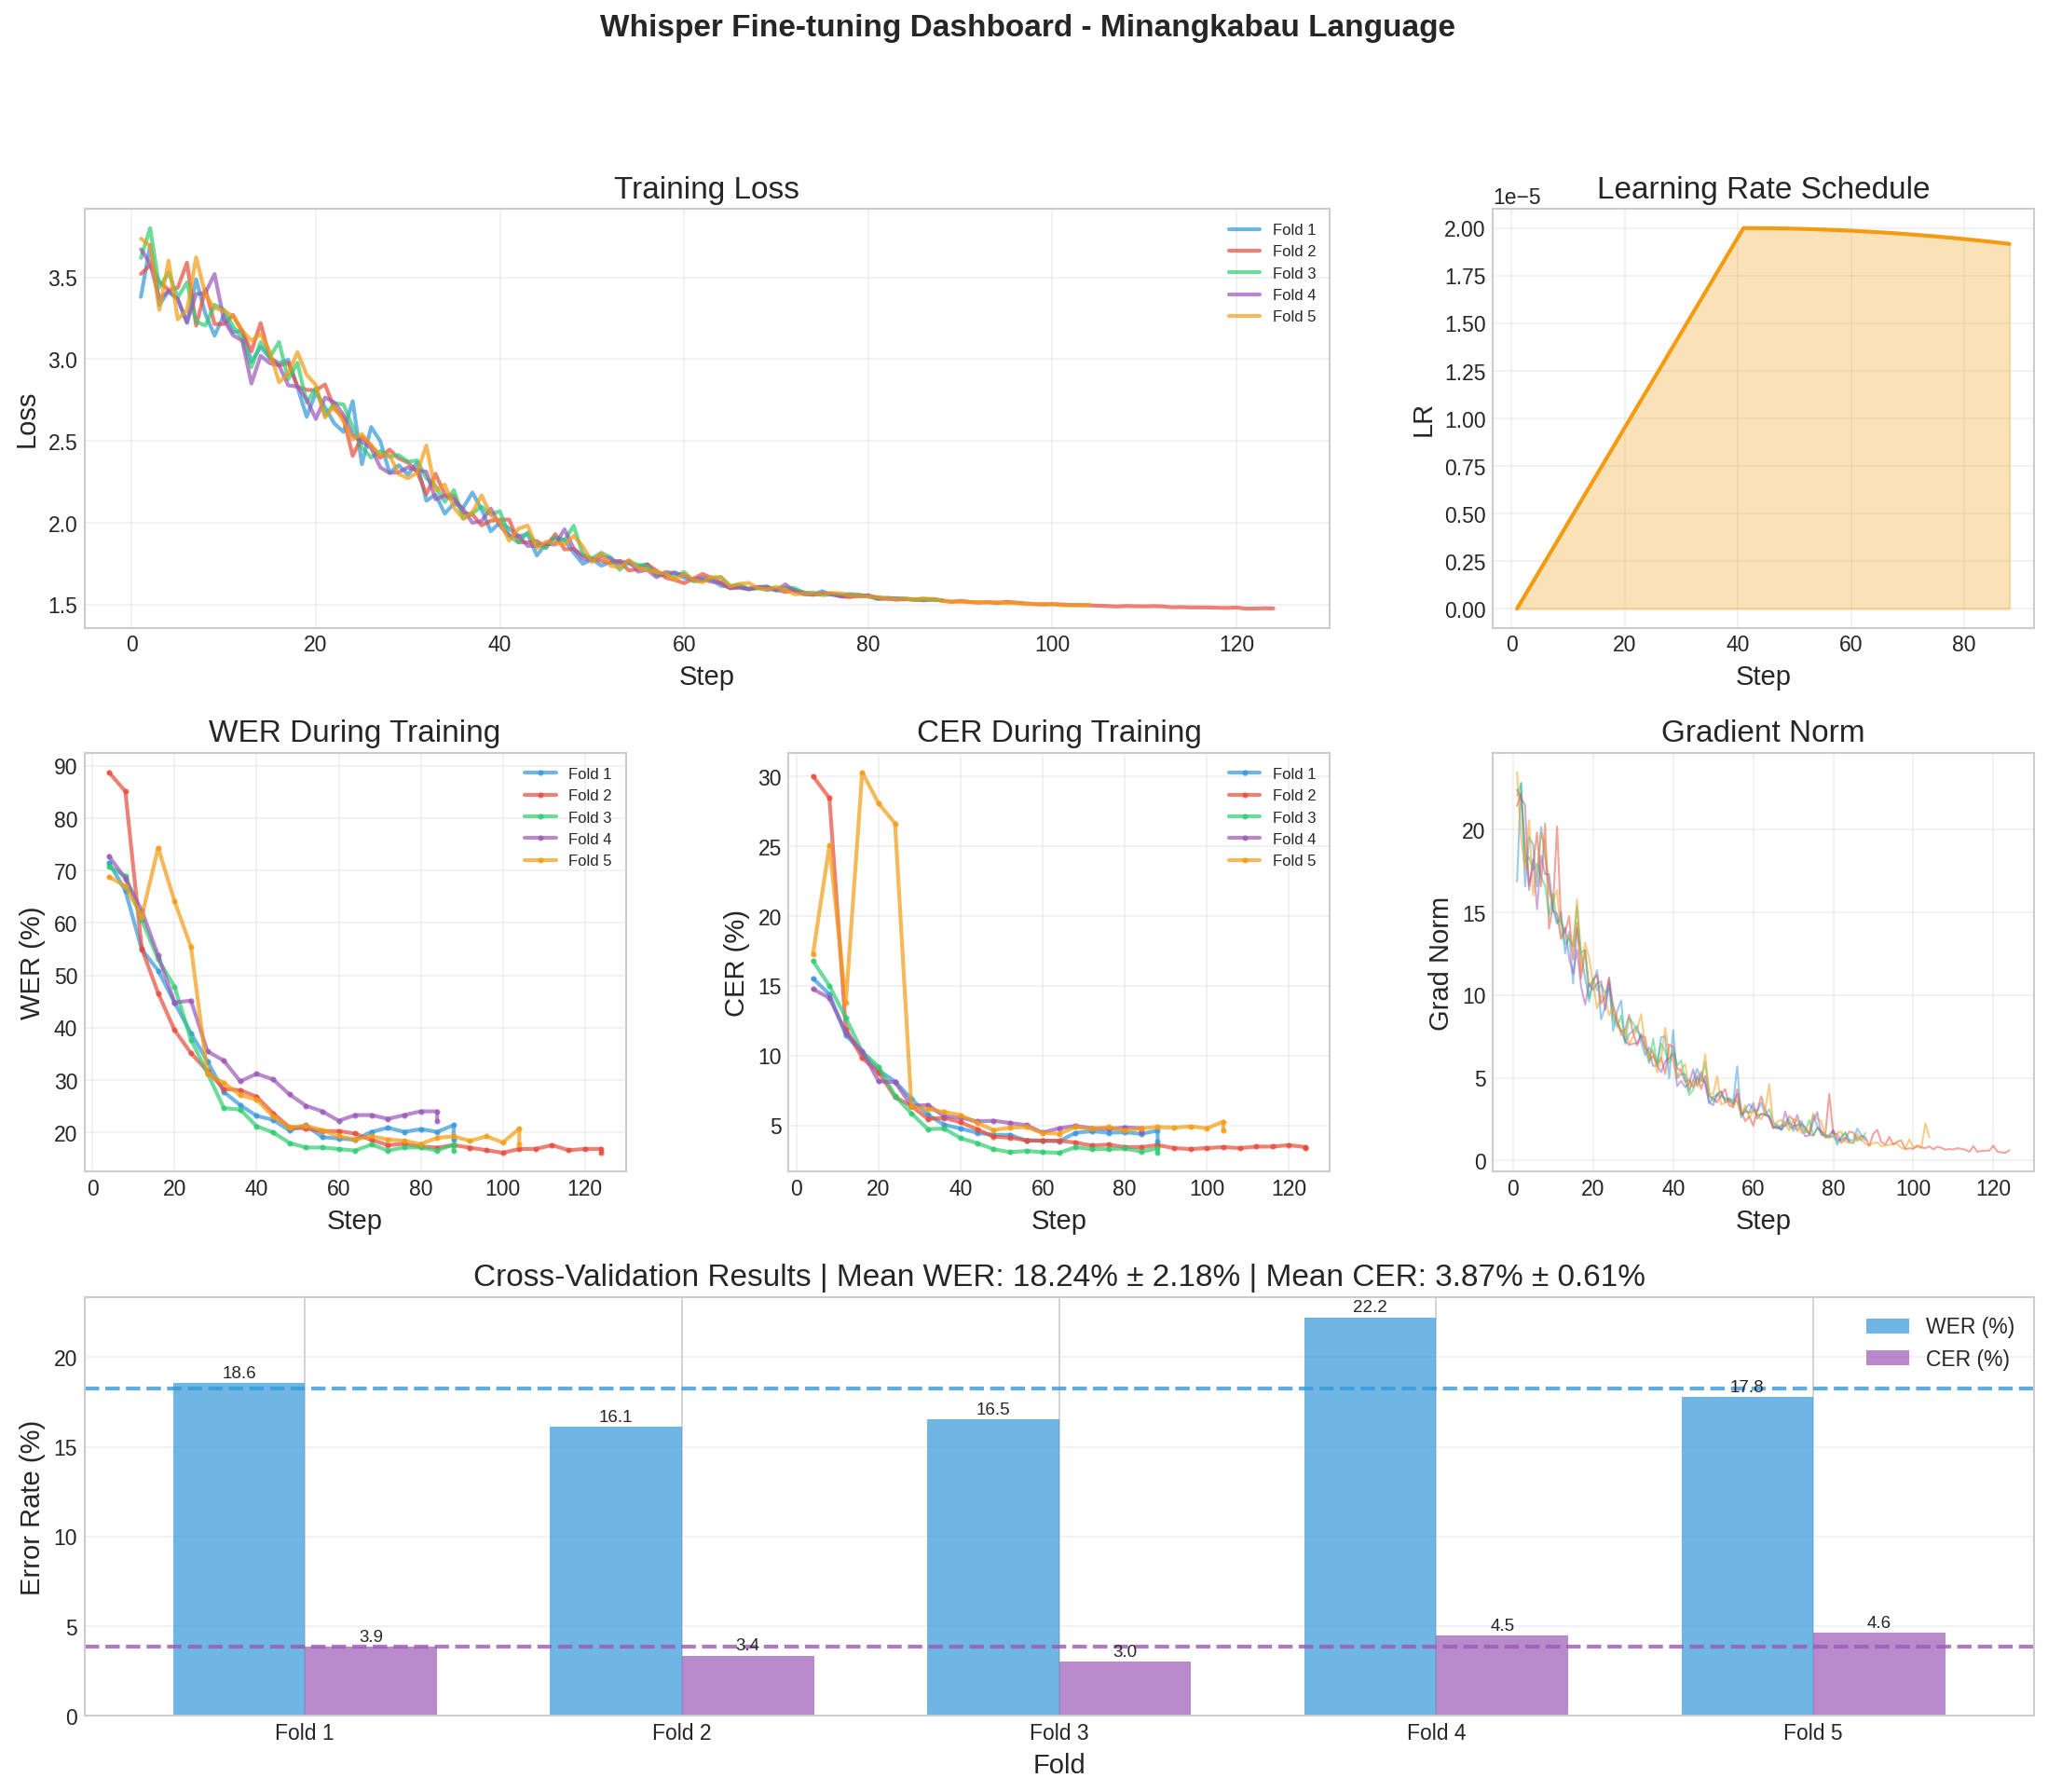
\includegraphics[width=\textwidth,height=5cm]{../code/freeze_encoder/outputs/metrics/run_20260303_202534/visualizations/comprehensive_dashboard.png}
            \end{figure}
        \end{column}
        \begin{column}{0.5\textwidth}
            \textbf{LoRA (lora\_20260305\_205845)}
            \begin{figure}
                \centering
                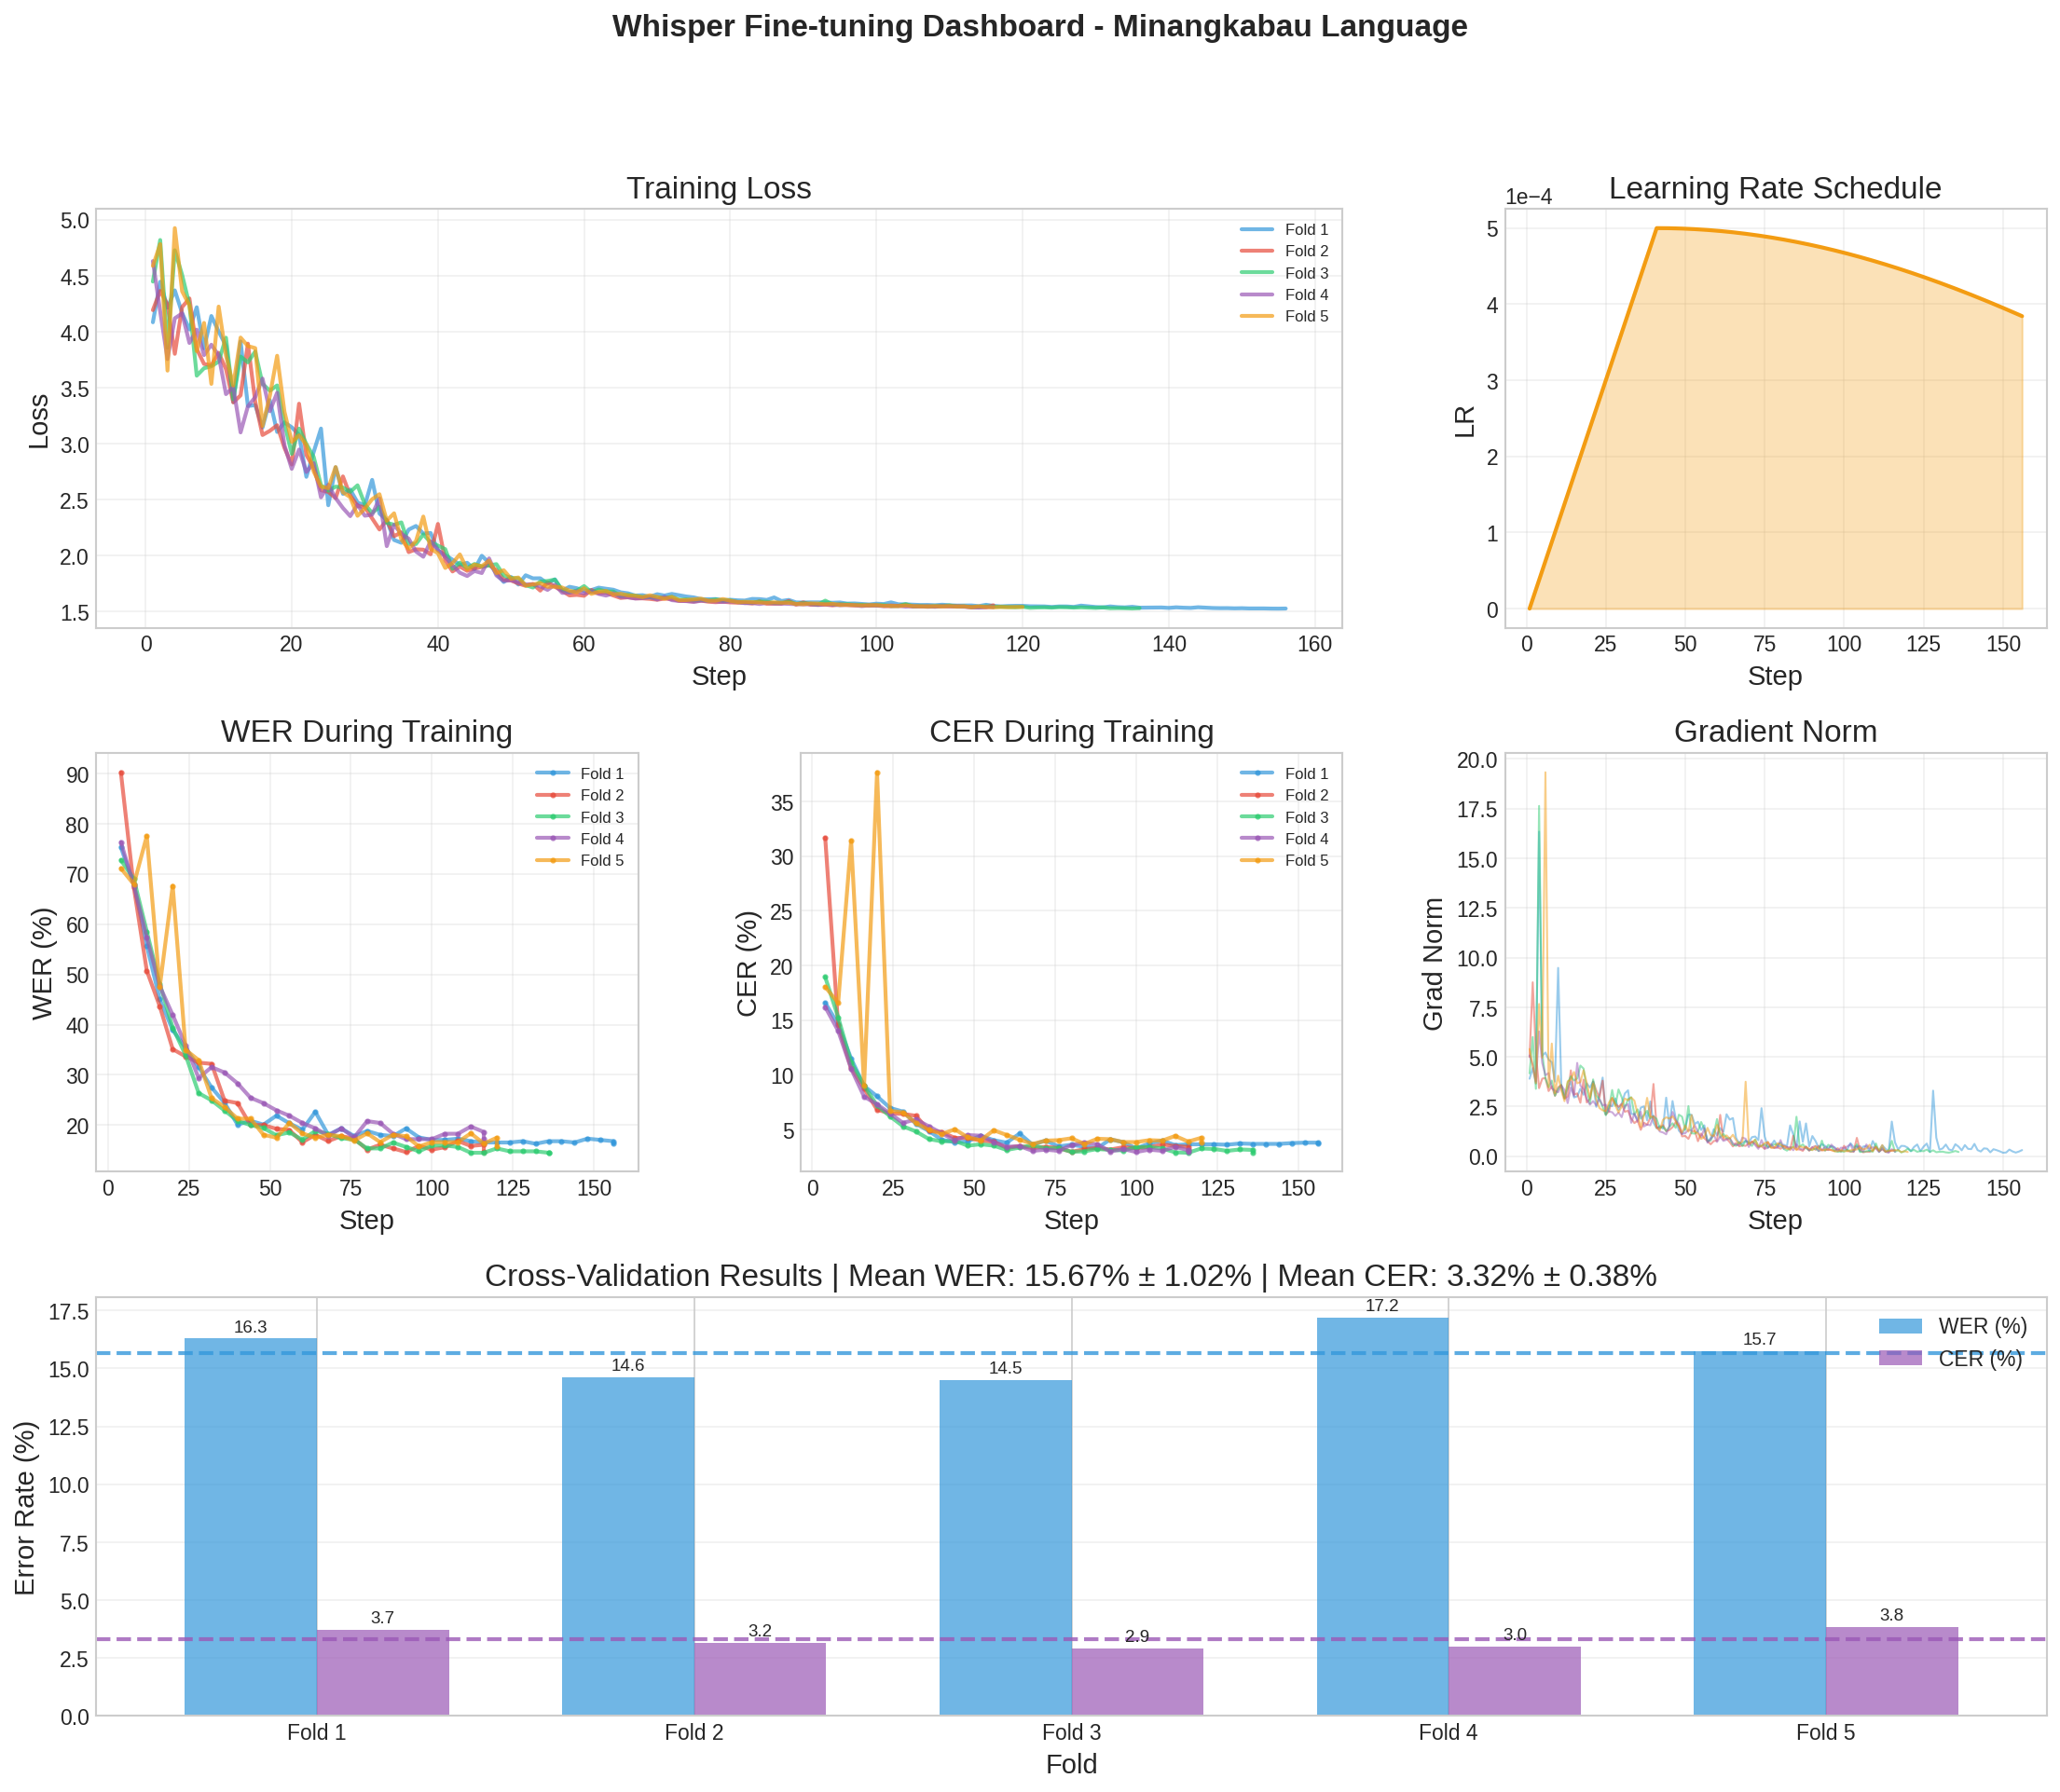
\includegraphics[width=\textwidth,height=5cm]{../code/lora/outputs/metrics/lora_20260305_205845/visualizations/comprehensive_dashboard.png}
            \end{figure}
        \end{column}
    \end{columns}
    \vspace{0.2cm}
    \small Dashboard menunjukkan LoRA lebih stabil antar-fold, terutama pada sebaran WER dan CER.
\end{frame}

\begin{frame}{Progres Kurva Loss dan Konvergensi Pelatihan}
    \begin{columns}
        \begin{column}{0.5\textwidth}
            \centering
            \textbf{Kurva Loss Freeze Encoder (FE terbaik)}
            \begin{figure}
                \centering
                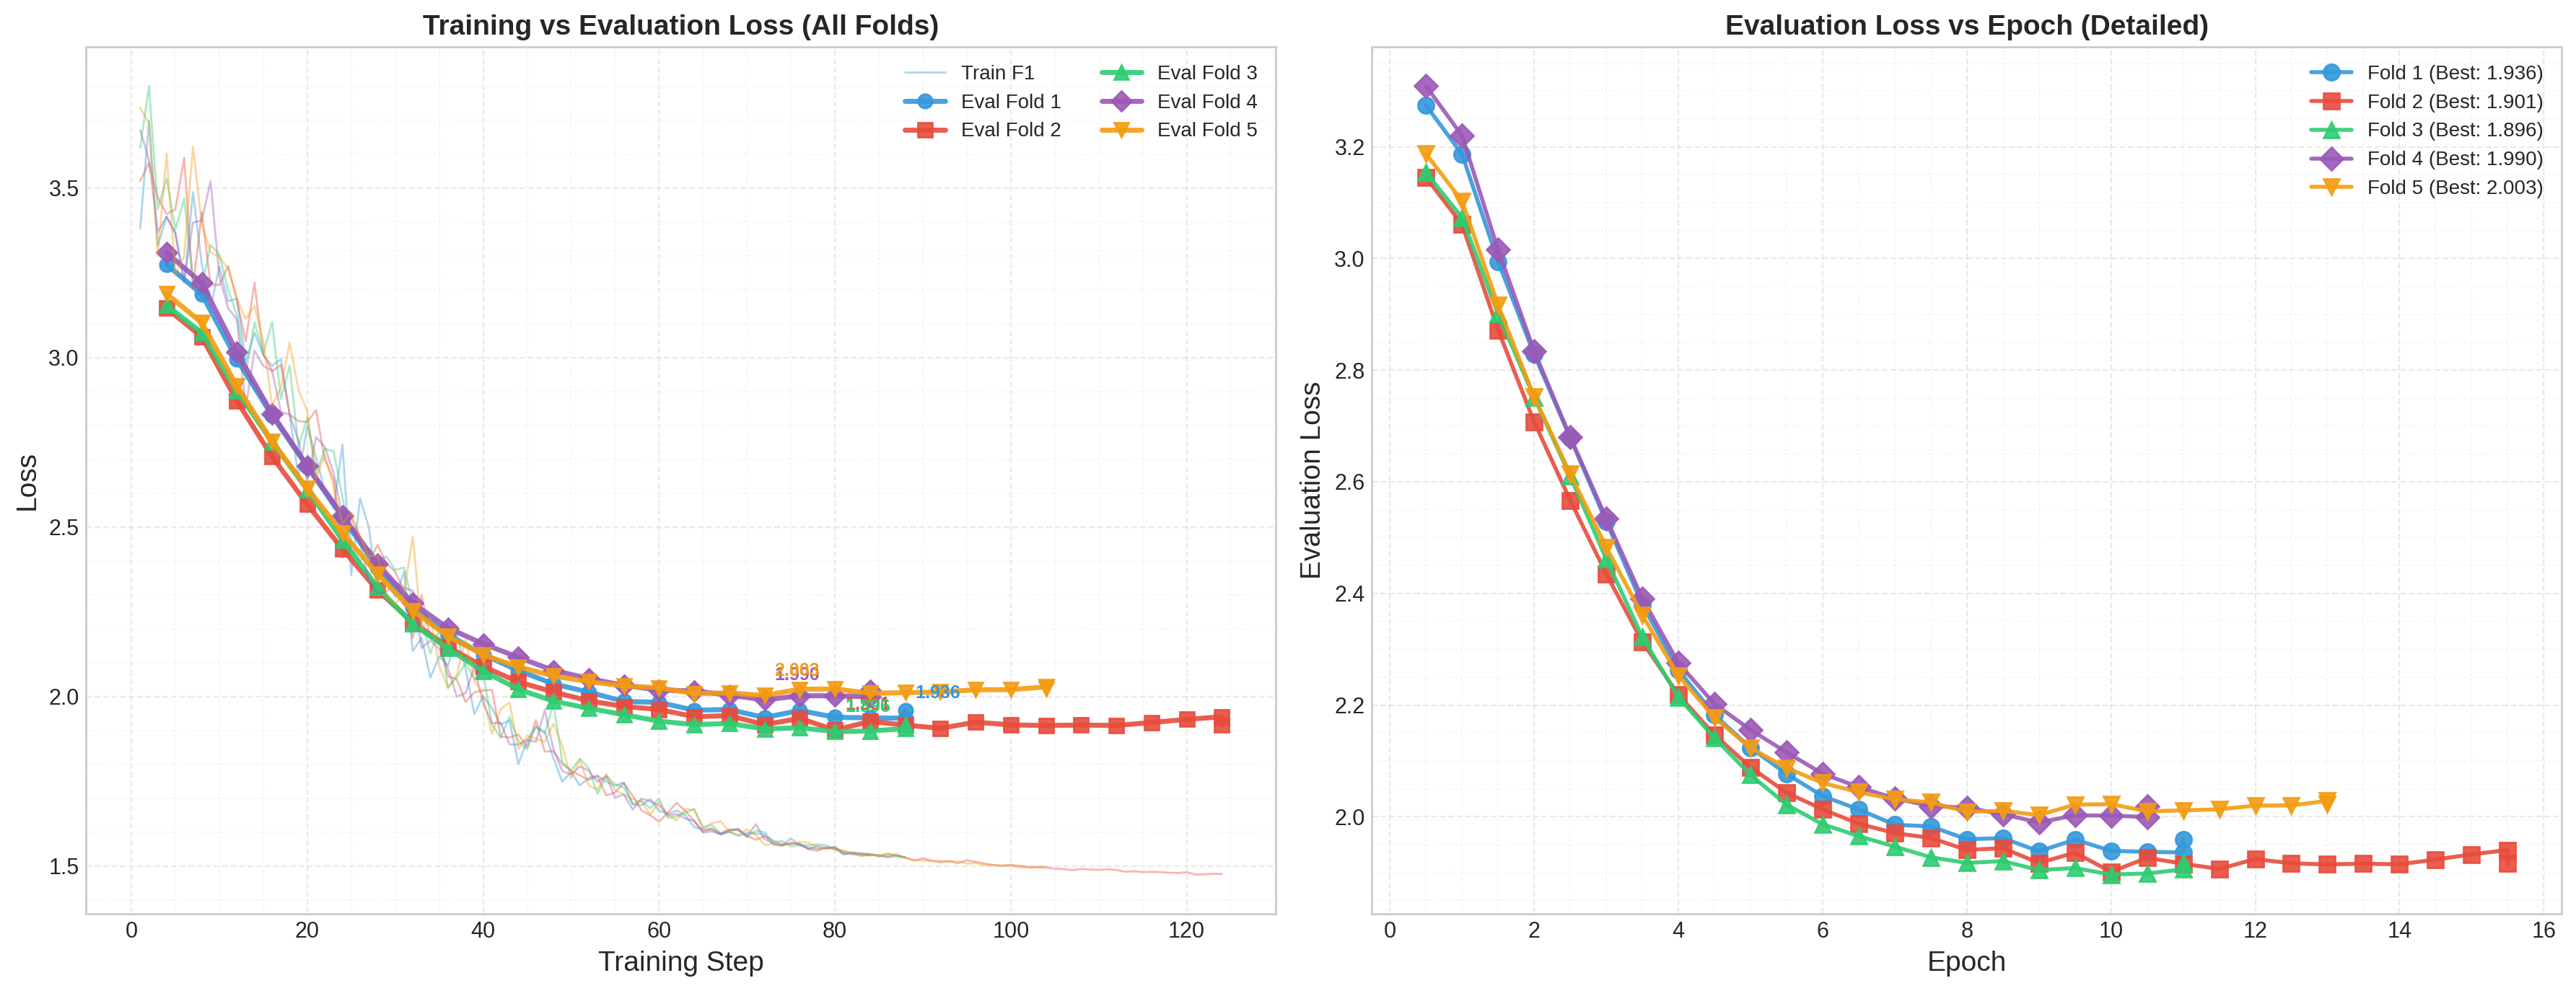
\includegraphics[width=\textwidth,height=4.5cm,keepaspectratio]{../code/freeze_encoder/outputs/metrics/run_20260303_202534/visualizations/loss_comparison_detailed.png}
                \caption{Fluktuasi Loss Train vs Eval FE terbaik}
            \end{figure}
        \end{column}
        \begin{column}{0.5\textwidth}
            \centering
            \textbf{Kurva Loss LoRA (LoRA terbaik)}
            \begin{figure}
                \centering
                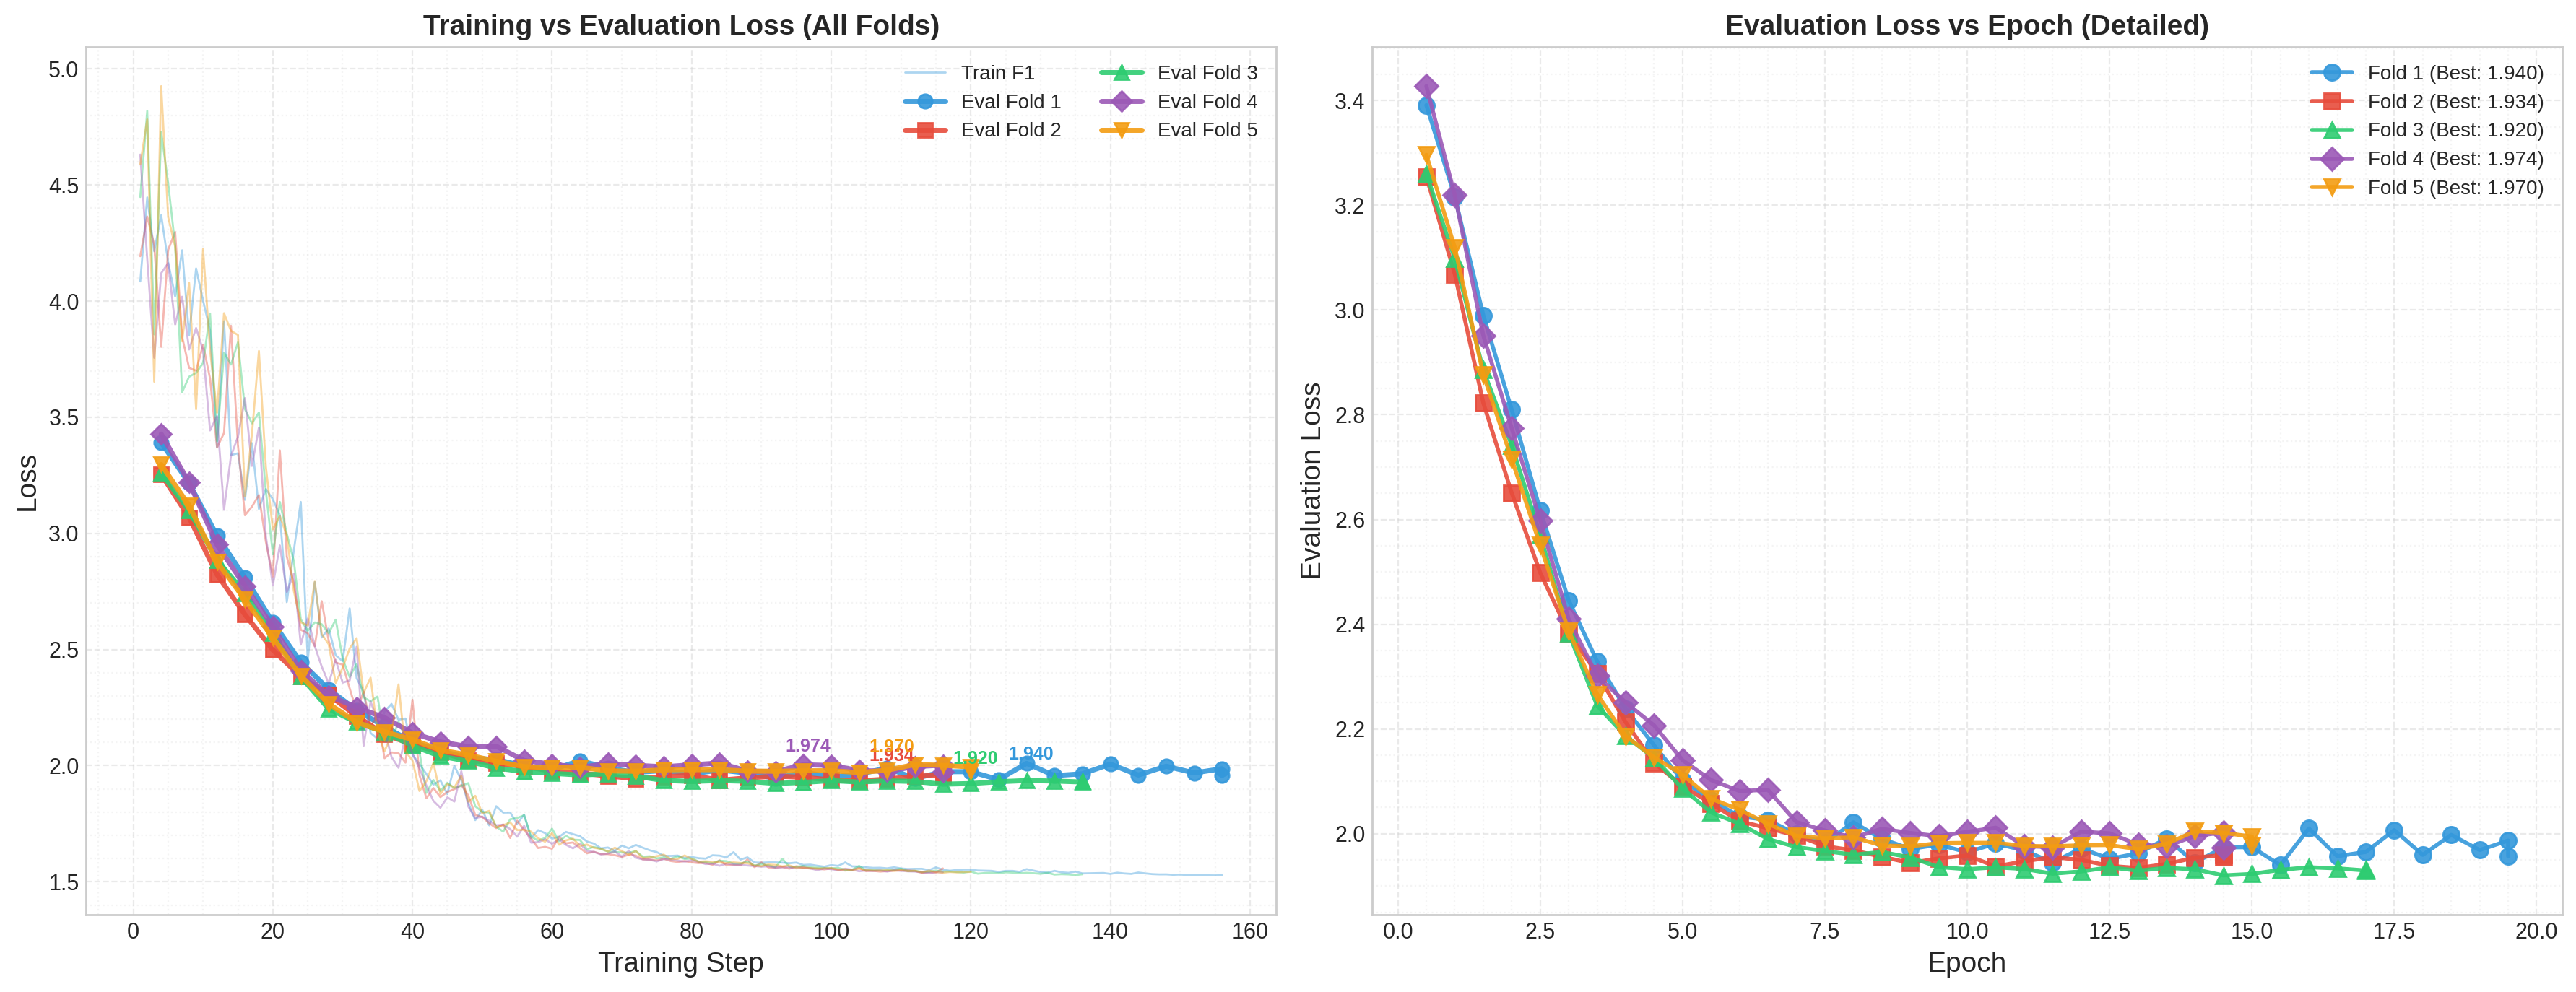
\includegraphics[width=\textwidth,height=4.5cm,keepaspectratio]{../code/lora/outputs/metrics/lora_20260305_205845/visualizations/loss_comparison_detailed.png}
                \caption{Konvergensi Loss Train vs Eval LoRA terbaik}
            \end{figure}
        \end{column}
    \end{columns}
    \vspace{0.2cm}
    \small Kurva \textit{loss} menunjukkan konvergensi LoRA yang lebih stabil pada 5-fold validasi dibandingkan Freeze Encoder.
\end{frame}

\begin{frame}{Dinamika Pelatihan LoRA Terbaik: Learning Rate \& Gradient Norm}
    \vspace{-0.2cm}
    \begin{columns}
        \begin{column}{0.5\textwidth}
            \textbf{Penjadwalan LR Cosine LoRA ($\alpha = 5\times10^{-4}$)}
            \begin{figure}
                \centering
                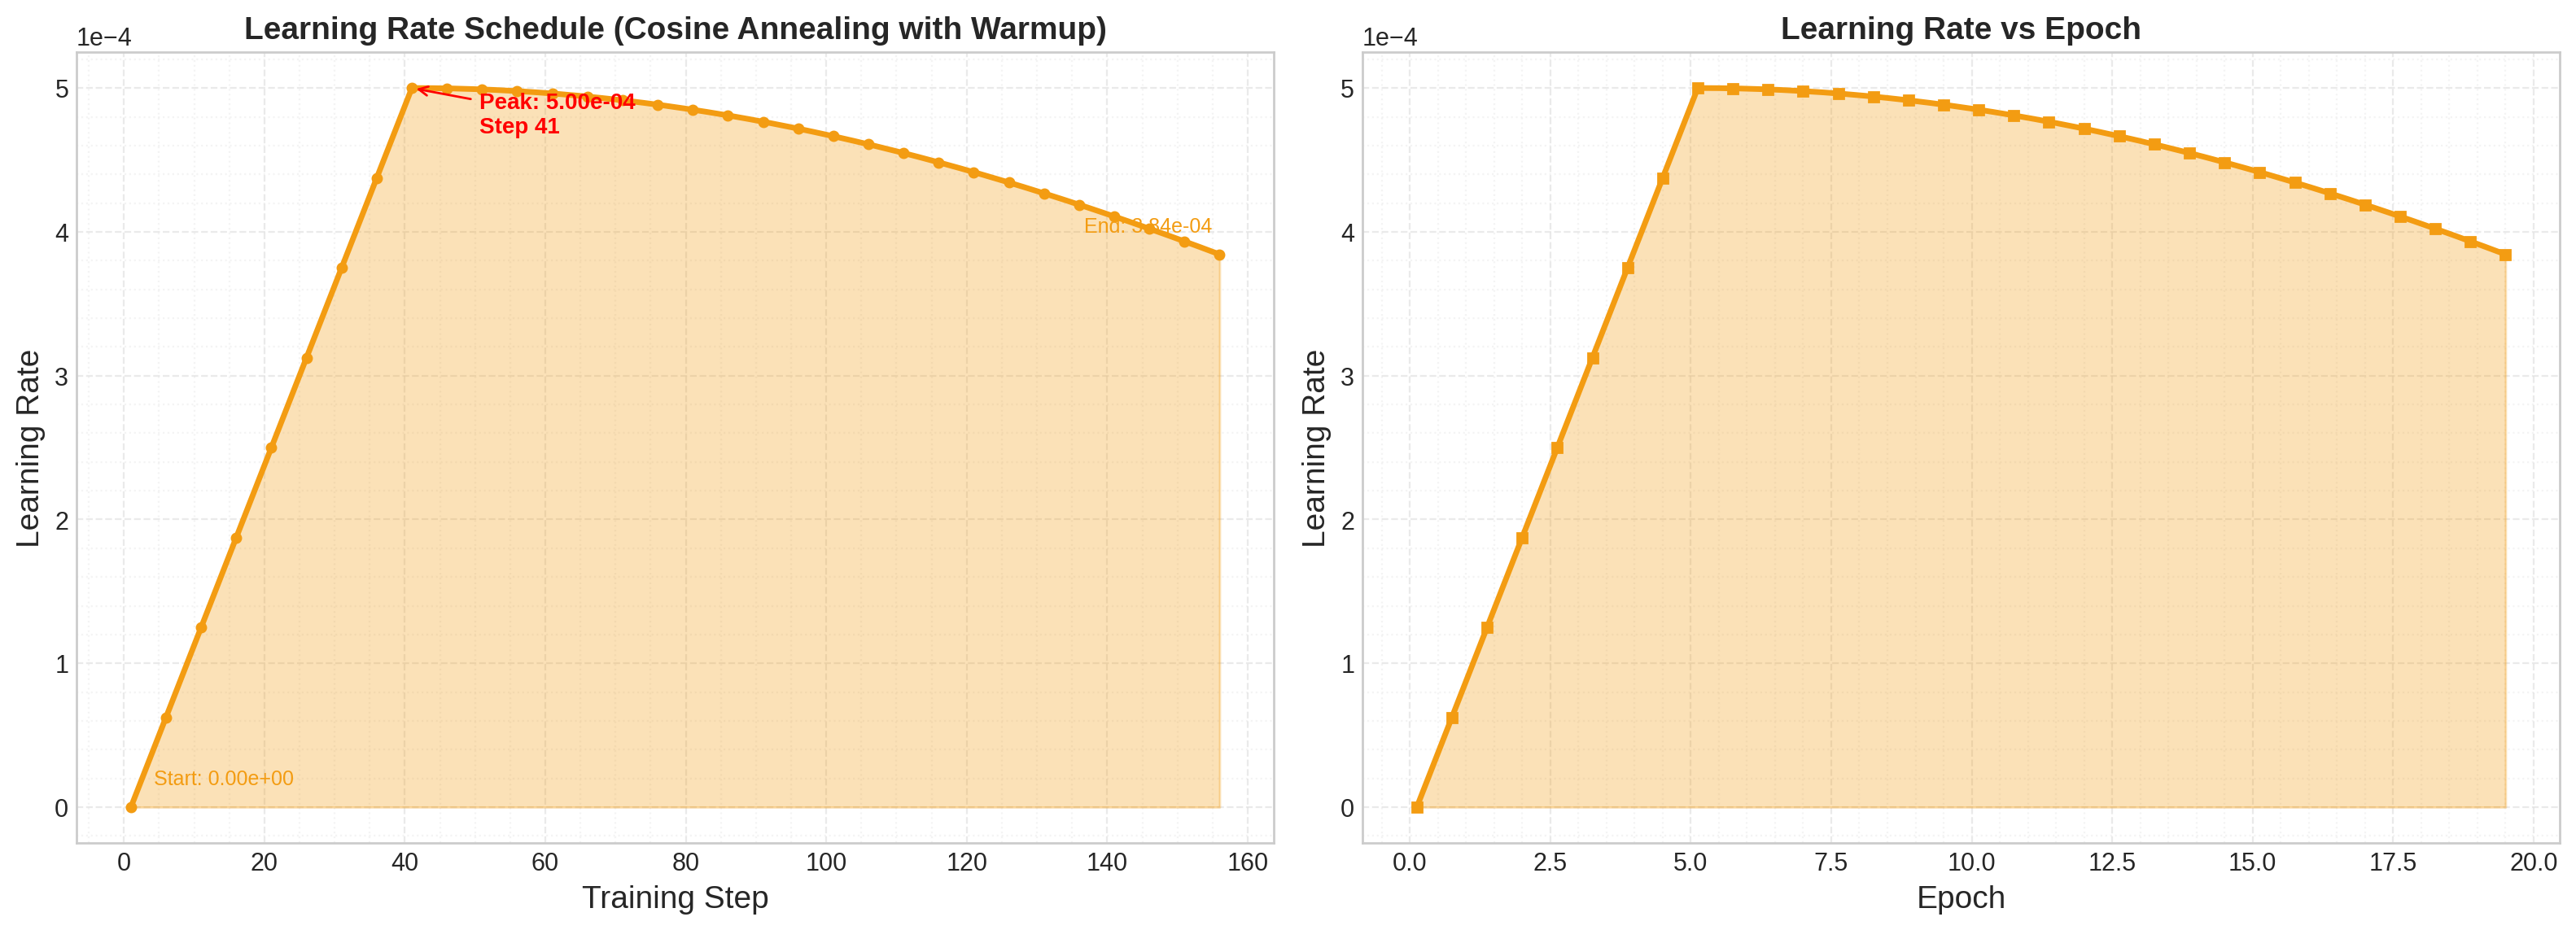
\includegraphics[width=\textwidth,height=4cm]{../code/lora/outputs/metrics/lora_20260305_205845/visualizations/learning_rate_schedule_detailed.png}
                \caption{Jadwal Learning Rate LoRA pada 5-fold}
            \end{figure}
        \end{column}
        \begin{column}{0.5\textwidth}
            \textbf{Norm Gradien Global Model LoRA}
            \begin{figure}
                \centering
                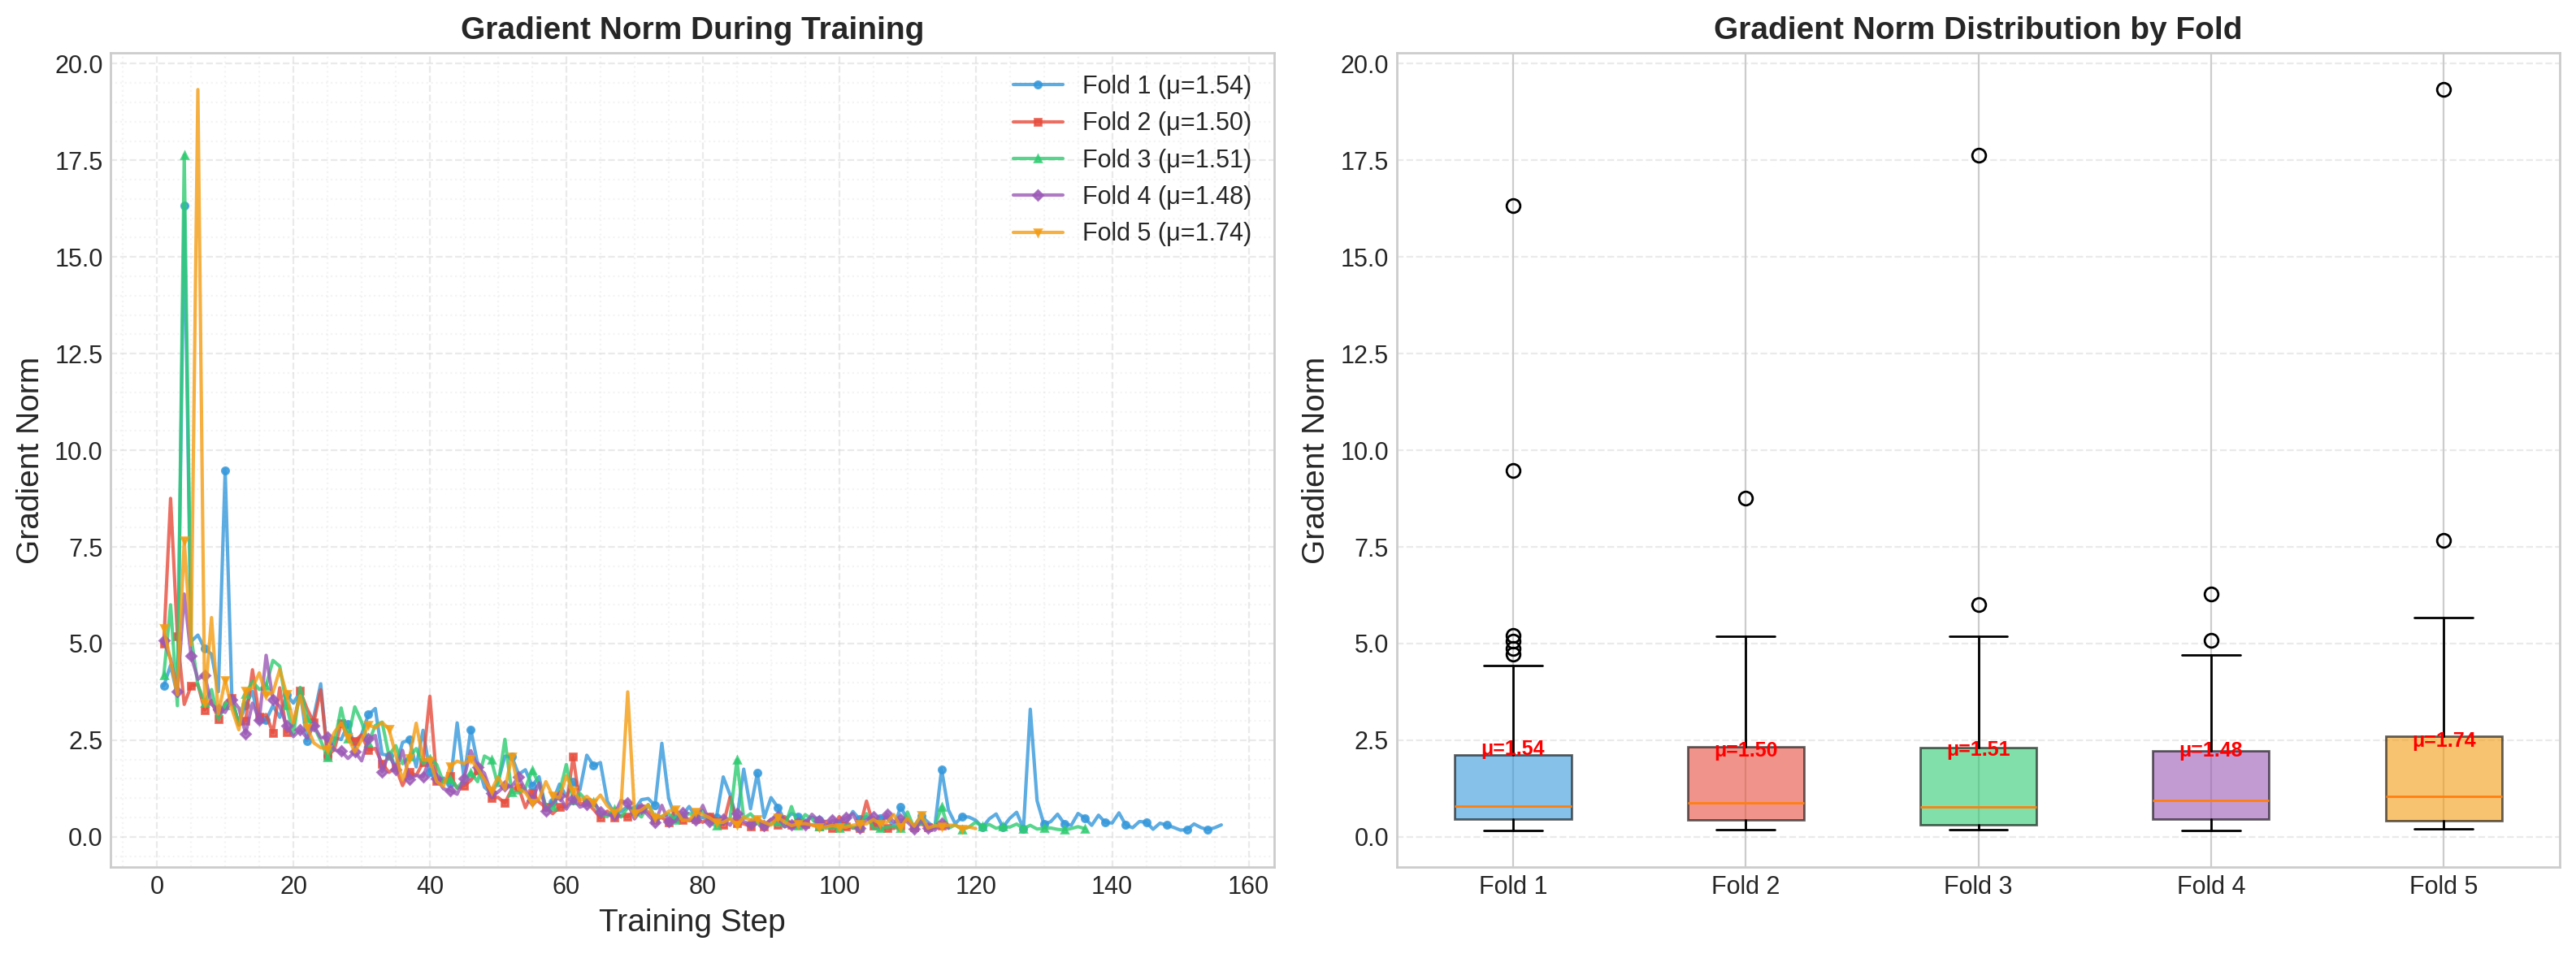
\includegraphics[width=\textwidth,height=4cm]{../code/lora/outputs/metrics/lora_20260305_205845/visualizations/gradient_norm_detailed.png}
                \caption{Stabilitas norm gradien LoRA pada 5-fold}
            \end{figure}
        \end{column}
    \end{columns}
    \vspace{0.2cm}
    \small Kedua grafik berasal dari run LoRA terbaik (\texttt{lora\_20260305\_205845}) dan menunjukkan peluruhan LR yang halus serta norm gradien yang stabil selama pelatihan 5-fold.
\end{frame}

\begin{frame}{Analisis Kesalahan Pasca-Training (Kualitatif)}
    Penjabaran kualitatif menunjukkan 3 permasalahan bahasa daerah:
    
    \begin{block}{1. Substitusi Fonetik karena Variasi Bunyi Analog}
        Penggantian bunyi konsonan antar pengguna bervariasi luas.
        \begin{itemize}
            \item Asli: \textit{panghormatan} $\rightarrow$ Prediksi: \textit{pangormatan} (huruf \textit{h} tidak terdengar tebal).
            \item Asli: \textit{dasar} $\rightarrow$ Prediksi: \textit{tasar} (Konsonan lemah).
        \end{itemize}
    \end{block}

    \begin{alertblock}{2. Segmentasi Kosakata (Tidak ada Pengejaan Baku)}
        Kata sering terpotong atau terhubung (\textit{Word Boundaries Blur}).
        \begin{itemize}
            \item Asli: \textit{mukadimah} $\rightarrow$ Prediksi: \textit{muka di ma}.
            \item Asli: \textit{hak-hak} $\rightarrow$ Prediksi: \textit{hak hak} (tanpa sepasang tanda strip).
        \end{itemize}
    \end{alertblock}

    \begin{exampleblock}{3. Halusinasi Model Autoregresif}
        Ketik dihadapkan dengan jeda diam \textit{prolonged silence}, atensi model sering menyantumkan gibberish dekoder dari kata lampau.
    \end{exampleblock}
\end{frame}